\section{強化学習の基本と初期の学習アプローチ}
本章では,本研究において採用された強化学習および適用された学習手法について説明する.さらに,参照したGitHub上のカーレースAIサンプルおよびその成果と課題についても開設する.
\subsection{強化学習の基礎と学習サイクル}
強化学習(Reinforcement learning)は,エージェントが環境の状態を観察し,どのように行動すれば最大の報酬を獲得できるかを学習する手法である.強化学習のサイクルは以下のように進行する.
\begin{enumerate}
  \item 状態取得:エージェントは環境を観察し,その状態を取得する.
  \item 行動決定:エージェントは,観察した状態に基づいてポリシーに従って行動を決定する.
  \item 行動実行:エージェントは,決定された行動を実行する.
  \item 報酬取得:行動の結果として,エージェントは報酬を受け取る.
  \item ポリシー更新:獲得した報酬と経験に基づき,ポリシーを更新する.
\end{enumerate}

最終的に,エージェントはこのサイクルを繰り返し,将来的に多くの報酬を得るためのポリシーを見つけ出す.

\subsection{エージェントの行動タイプ} 
強化学習サイクルでは,エージェントは取得した環境の状態に応じてエージェントが行動を選択する.行動には,連続値(Continuous)と離散値(Discrete)の2つの型がある.「Continuous」の場合,-1.0 から 1.0のような連続した値を取る浮動小数点数の配列を行動として使用する.一方,「Discrete」の場合は,0,1,2 のような離散した値を持つ整数配列を行動として使用する.本研究で使用したGitHubのカーレースAIサンプルでは「Continuous」型の行動が採用されているが,第3章「スクラッチから学習環境の構築」では,「Discrete」型の行動を用いた.サンプルのカーレースAIの実装結果に基づき,「Continuous」型では浮動小数点数を用いるため操作の選択肢が非常に多く,初期段階で経験のないエージェントにとって学習が難しく,失敗する可能性が高かまる.一方で,「Discrete」型では離散が限られているため,エージェントの学習を容易に進めることが可能になる.

\subsection{使用した学習手法}
Unity ML-Agentsでは,「PPO」と「SAC」の2つの強化学習アルゴリズムが利用可能である.ハイパーパラメータの設定項目は,使用するアルゴリズムが「SAC」か「PPO」かによって異なる.
「SAC」(Soft Actor-Critic)はオフポリシーのアルゴリズムであり,過去の経験から学習を促進する.一方,「PPO」(Proximal Policy Optimization)はオンポリシーのアルゴリズムで,現在のポリシーに基づいて学習を進める.PPOは,学習過去の安定性を高めるために,ポリシーの急激な変更を抑制する特徴がある.
本研究では,カーレースAIのサンプルおよびスクラッチから構築した学習環境において,「PPO」アルゴリズムを用いて学習を行った.

\subsection{エージェントの環境認識:観察とセンサー}
カートの学習において,初期段階ではカートがランダムに動きながらトラックを探索する.この探索は,カメラではなく,周囲の環境を認識するためにRaycast 3D センサーを使用した.Unityでは,2Dおよび3Dの環境で使用可能なRaycastセンサーがあるが,本研究では3Dの環境で学習を行うため,Raycast 3D センサーを使用した.

\subsection{エージェントクラスのオーバーライドメソッド}
エージェントのスクリプトでは,エピソード開始時の初期化,観察の取得,行動の実行と報酬の取得などを実装する.以下に,本研究で使用されたいくつかの重要なエージェントクラスを説明する.
\begin{enumerate}
  \item \textbf{OnEpisodeBegin() の追加:}エピソードが開始する際に実行される関数である.
  \item \textbf{CollectObservations() の追加:}エージェントが観察を収集する関数である.引数 'VectorSensor' の 'AddObservation()' メソッドを使用して,観察の値をエージェントに渡す.
  \item \textbf{OnActionReceived() の追加:}決定された行動に基づいて行動を実行する.
\end{enumerate}

この3つのメソッドは,学習用スクリプトを作成する際に特に重要視された.また,これらの設定に関する詳細は,後述の「サンプルの実行の詳細」と「学習用のエージェントスクリプト」のセクションで説明される.

\subsection{サンプル実行の詳細}
\subsubsection{サンプルの学習環境}
カーレースゲームのサンプルは,GitHubで公開されているレーシングゲームのサンプル\cite{AI-Racing-Karts}を基にしている.
学習の初期段階では,公開されているトラックを使用し,カートを配置して学習を開始した.学習プロセスを高速化するために,複数のカートをトラック上に配置した.

また,使用したカーレースAIサンプルの学習環境におけるトラックレイアウトやカートのモデルを,図1と図2に示す.

\begin{figure}[H]
    \centering
    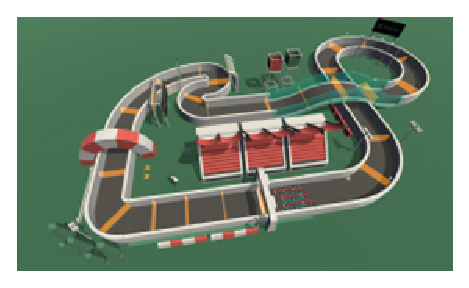
\includegraphics[width=0.8\textwidth]{figures/TrackLayout.eps}
    \caption{カーレースAIサンプルの学習環境【トラックのレイアウト】}
    \label{fig:sample-environment}
\end{figure}

\begin{figure}[H]
    \centering
    \includegraphics[width=0.8\textwidth]{figures/KartModel.eps}
    \caption{カーレースAIサンプルの学習環境【カートのモデル】}
    \label{fig:kart-model}
\end{figure}

\subsubsection{学習用のスクリプト}
カートを動かすためのスクリプトに加えて,学習するためのエージェントスクリプトが追加された.このスクリプトには,エージェントが行う行動に対して報酬の設定を追加した.行動のタイプは「Continuous」に設定された.これは,浮動小数点数を使用することでカートの動きをより滑らかに制御できるためである.報酬の設定では,トラック上に見えないチェックポイントを配置し,これを正しく通過すると報酬が与えられる.また,カートが誤ったチェックポイントを通過するとペナルティとしてマイナスの報酬を与えるように設定された.学習プロセスを効率的に進めるため,20ms ごとに小さなマイナスの報酬を適用した.

Unity ML-Agentsを用いた学習プロセスは,'mlagents-learn' コマンドと学習設定ファイルを使用して行われる.このプロセスを通じて,コマンドライン引数と学習設定ファイルのパラメータに基づいて学習が実施される.

\subsubsection{学習結果と考察}
カーレースAIサンプルの学習結果はTensorboardで閲覧することができ,累計報酬とエピソードの長さの詳細が確認できる.その学習結果を以下の図3に示す.

\begin{figure}[H]
    \centering
    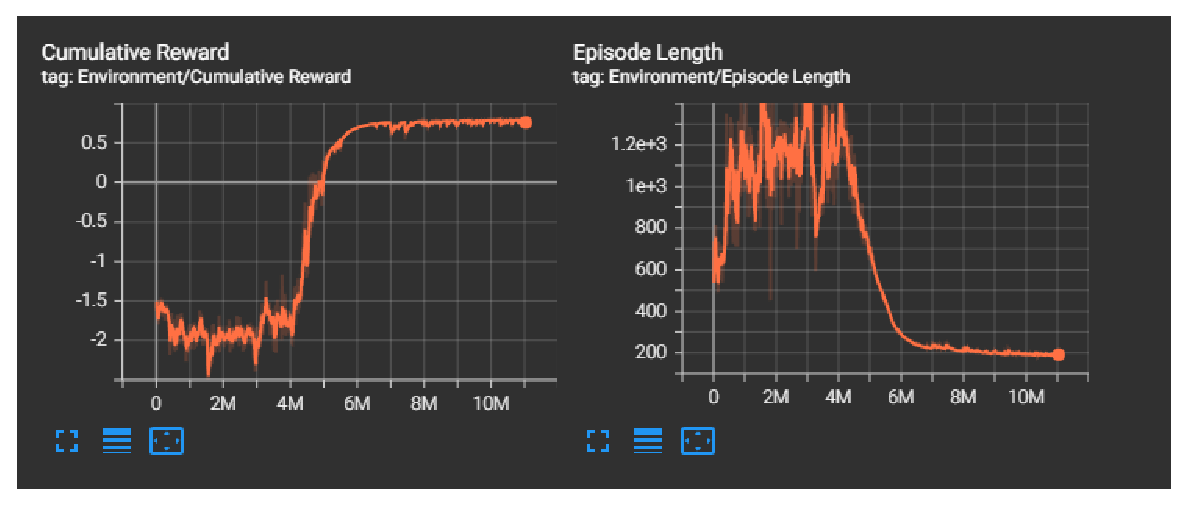
\includegraphics[width=1\textwidth]{figures/Tensorboard.eps}
    \caption{カーレースゲームサンプルの結果}
    \label{fig:sample-graph}
\end{figure}


図3からわかるように,400万ステップの学習を実施した結果,初期は累計報酬がマイナスであったものの,250万ステップ目以降に累計報酬が著しく向上した.報酬の向上に伴い,エピソードの長さも短縮されていることが確認できた.

しかし,この学習結果にはいくつかの問題点があった.学習の初期段階では,カートが後退し続けることで累計報酬が改善されず,学習プロセスを何度も中断せざるを得なかったこと,カートの動きが現実の車とは異なり,停止状態でも左右に回転できるため不自然であったこと,そしてカートが壁に衝突する問題があったことである.壁に衝突した際のペナルティが導入されていなかったため,カートが壁を利用して前進し続けた.結果として,カーレースAIのサンプルでは壁に衝突せずに走行することは実現できなかった.

上記の問題点をすべて改善するため,スクラッチから新しい学習環境を構築することにした.この新しい学習環境,その構築過程,および学習結果については,以下の第3章以降で詳しく説明する.
